En este ejercicio dado un buque mercante cuya capacidad de carga es de K toneladas y un conjunto de contenedores $c_1,...,c_n$ cuyos
pesos respectivos son $p_1,...,p_n$, debemos hallar un algoritmo que maximice el número de contenedores cargados y otro que intente 
maximizar el número de toneladas cargadas.

\subsection{Maximización de contenedores}

En primer lugar, debemos ser conscientes de que la capacidad del buque debe ser menor que la suma total de los pesos 
de los contenedores, pues en caso contrario, no estaría bien definido el problema. Para resolver este problema tenemos que darnos cuenta
que lo que nos interesa es ir cogiendo aquellos contenedores cuyo peso sea más pequeño e ir introduciéndolos en el buque mientras que su suma 
sea menor que la capacidad de carga del buque, puesto que el resultado debe tener el mayor número de contenedores posible, sin importar las 
toneladas totales. Una ilustración del objetivo que queremos conseguir se puede observar en Figura~\ref{fig:dib1}. 

\begin{figure}[H] 
    \centering
    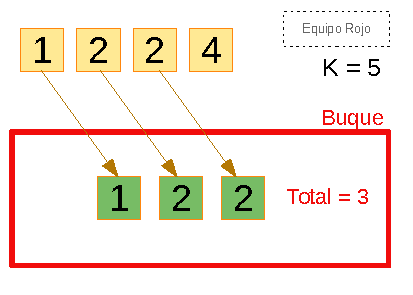
\includegraphics[scale=1]{img/DibCont1.pdf}
    \caption{Ilustración de la maximización del número de contenedores.}
    \label{fig:dib1}
\end{figure}

\subsubsection{Pseudocódigo}

\begin{algorithm}[H]
    \caption{Algoritmo para maximizar el número de contenedores}\label{alg:max_containers}
    \begin{minipage}{0.92\textwidth}
    \textbf{Parámetro}: contenedores (vector de enteros)

    \textbf{Parámetro}: K (capacidad del buque)

    \end{minipage}

    peso = 0\;
    vector resultado\;
    lleno = false\;

    sort(pesos.begin(), pesos.end());

    \For{i desde 0 hasta contenedores.tamaño-1 y !lleno} {
        \eIf{contenedores$[i]$ + peso $\leq$ K}{
            peso += contenedores$[i]$\;
        }{ lleno = true\;}
    }

    \Return{result}
    
\end{algorithm}

Como vemos en el algoritmo la clave del proceso es antes de añadir los contenedores, ordenarlos de forma creciente para que 
en el ciclo siempre se vaya añadiendo el contenedor con menor peso. 
Para llevar a cabo la implementación de este algoritmo, según lo visto en clase, lo hemos dividido en ciertas funciones que 
determinarán la condición de factibilidad y de solución, mientras que lo demás lo hemos unificado todo en una función. 

\subsubsection{Implementación}

\lstinputlisting[label={cod:max_containers}, firstline=8, lastline=47, language=C++,
caption=Implementación del algoritmo del máximo de contenedores.]{../src/ejercicio-1-a.cpp}

\subsubsection{Análisis de Eficiencia}

Para el análisis de eficiencia, llamamos $n$ a la cardinalidad del vector de pesos, nos situamos en la función \texttt{nContenedoresMax}, observamos que realizamos una llamada a \texttt{sort} de eficiencia $O(nlog(n))$, y posteriormente tenemos un bucle \texttt{while} que en el peor de los casos recorrerá el vector de pesos, y las llamadas a \texttt{esFactible} y \texttt{esSolucion} son $O(n)$, luego la eficiencia del bucle es $O(n^2)$. Por tanto, la eficiencia total del algoritmo es $O(n^2)$.

\subsubsection{Condición de optimalidad}
En esta sección discutiremos si el algoritmo presentado es óptimo. Veremos que,
efectivamente, la estrategia greedy maximiza el número de contenedores 
en la solución final que se ha propuesto. 

\textbf{Notación.} Sean $K$ la capacidad máxima de carga del buque y
$P = \{p_1,p_2,\cdots,p_n\}$ el conjuntos de pesos asociados
a los contenedores. Consideramos $\mathcal{S} = \{S \subset P : 
\sum_{p \in S} p \leq K\}$ el conjunto de soluciones. Decimos que una solución
$T \in \mathcal{S}$ es \textbf{óptima} cuando se verifica que $|S| \leq |T|,
\forall S \in \mathcal{S}$. 
También diremos que un conjunto $W$ es una \textbf{solución parcial}
si verifica que $\exists S \in \mathcal S$ tal que $W \subset S$. Sea $\mathcal{W}$ 
la \textbf{familia} de todas las soluciones parciales.

Verificaremos varias propiedades, antes de realizar la demostración de la optimalidad.

\begin{lemma}
    Sea $\mathcal{S} = \{S \subset P : \sum_{p \in S} p \leq K\}$ el conjunto de soluciones. Entonces
    existe $S_m \in \mathcal S$ óptimo. 
\end{lemma}

\begin{proof}
    La demostración es bastante evidente. Como $|P| = n$, tenemos que $|\mathcal S| \leq |\mathcal P (P)| = 2^n$. 
    Empleando un algoritmo por fuerza bruta, podríamos probar todas las posibles combinaciones, determinando si
    son conjuntos que pertenecen a $\mathcal S$, de donde $\mathcal S$ es finito por ser un subconjunto de un conjunto finito. 
    Tenemos entonces que $\{|S| : S \in \mathcal S\}$ es finito, por lo que existe $S_m \in \mathcal S$ tal que
    $|S| \leq |S_m|, \forall S \in \mathcal S$, de donde $S_m$ es óptimo, como queríamos. 
\end{proof}

% \begin{lemma}
%     Sea $m \in \mathbb N$ tal que $a_{m} = min\{W\}$, con W una solución parcial. Entonces existe $S_m \in \mathcal S$ óptimo tal que
%     $a_m \in S_m$. 
% \end{lemma}

% \begin{proof}
%     Sea $S \in \mathcal S$ una solución óptima. Veamos que llamando $a = \min\{S\}$, se verifica que
%     $S_m = W \backslash\{a\}\cup{\{a_m\}}$ es también una solución óptima. En efecto, $\sum_{p \in S_m} p \leq 
%     \sum_{p \in S} p \leq K$, por lo que $S_m \in \mathcal S$. Además, es claro que
%     $ |A| \leq |S| = |S_m|, \forall A \in \mathcal S$, por lo que $S_m$ es óptimo, con $a_m \in S_m$. 
% \end{proof}

% Nótese que este segundo lema es clave, pues admite la existencia de una solución óptima empleando
% el algoritmo greedy. Además, la propiedad de existencia no únicamente
% se aplica al problema original, sino que también se aplica a los subproblemas generados a
% partir del algoritmo greedy, donde se han tomado previamente n etapas greedy. 
% De esta manera, podemos concretar el teorema clave para la optimalidad.

% \begin{theorem}
%     El algoritmo greedy proporciona una solución $S_{n} \in \mathcal{S}$ óptima. 
% \end{theorem}

% \begin{proof}
%     Ya hemos visto que existe una solución óptima. Veamos que la estrategia greedy proporciona
%     una solución $S_n$ óptima. En virtud del algoritmo propuesto, es claro que 
%     $S_n \in \mathcal S$ (pues se trata de la condición de parada). Para la optimalidad,
%     procedemos por inducción. Para $n=1$, la solución es clara en virtud de los lemas
%     anteriores. Para $S_n$ un subconjunto donde se ha empleado el algoritmo greedy, tenemos que,
%     nuevamente por el lema anterior, $S_{n+1}$ también se trata de una solución óptima. 
% \end{proof}

\begin{lemma}
    Sea $W \in \mathcal W$ y sea $G_k$ un conjunto formado
    por la k primeros elementos escogidos mediante el algoritmo greedy. 
    Entonces se verifica $\sum_{p \in G_k} \leq \sum_{p \in W}$. 
\end{lemma}

\begin{proof}
    Sean $W = \{w_1,\cdots, w_k\}$ y $G_k = \{g_1,\cdots,g_k\}$ los conjuntos considerados.
    Podemos suponer, sin pérdida de generalidad, que se verifica
    $w_1 \leq w_2 \leq \cdots \leq w_k$ y $g_1 \leq g_2 \leq \cdots \leq g_k$. 
    Puesto que en el algoritmo greedy siempre se selecciona, en primer lugar, los elementos
    mínimos a considerar, tenemos que se verifica $g_i \leq w_i, \forall i \in \{1,2,\cdots,k\}$,
    de donde sumando miembro a miembro se tiene la desigualdad enunciada.

\end{proof}

Una vez demostradas las propiedades anteriores, podemos proceder con la condición
de optimalidad.

\begin{theorem}
    Sean $\mathcal{S} = \{S \subset P : \sum_{p \in S} p \leq K\}$ el conjunto de soluciones y
    $P = \{p_1,p_2,\cdots,p_n\}$ el conjuntos de pesos asociados
a los contenedores. 
    Sea $G \in \mathcal S$ la solución generada por el algoritmo greedy. Entonces
    $G$ es óptimo. 
\end{theorem}

\begin{proof}
    Por los lemas anteriores, deducimos que existe una solución $S \in \mathcal S$ óptima.
    Como es claro que $G \in \mathcal S$, para demostrar que $G$ también es óptimo, 
    basta realizar $k = n$ para el lema anterior, de donde $|G| = |S|$, por lo que
    $G$ es óptimo.
\end{proof}

\newpage

\subsection{Maximización de toneladas}
En este caso tenemos que maximizar las toneladas por lo que para ello una buena estrategia es ir cogiendo los valores 
de mayor a menor peso, sin terminar las iteraciones cuando el introducir un contenedor hace que se supere la capacidad del
buque, pues como nos interesa maximizar la carga podemos aumentarla con contenedores con pesos más pequeños, siempre y cuando 
estos sumados al peso existente no supere la capacidad del buque.

\subsubsection{Pseudocódigo}

\begin{algorithm}[H]
    \caption{Algoritmo para maximizar las toneladas}\label{alg:max_toneladas}
    \begin{minipage}{0.92\textwidth}

    \textbf{Parámetro}: containers (vector de enteros)

    \textbf{Parámetro}: K (capacidad del buque)

    \end{minipage}

    weight = 0\;
	container = 0\;
    vector result\;
  
    sort(containers.begin(),containers.end(),greater$<$int$>$());

    \While{$weight  \leq K$ y $container  \leq containers.size$}{      
        \If{$weight + containers.at(container) \leq K$}{
            result.push\_back(containers.at(container))\;
            $weight += containers.at(container)$\;
        }
        container++\;
    }
  

    \Return{result}
\end{algorithm}

En este apartado también hemos divido la función principal encargada de hallar el máximo de toneladas, en varias funciones
booleanas, una para determinar si una solución es factible y otra para ver si puede ser solución. Todo ello para distinguir 
las características de un algoritmo greedy en nuestro código.

\subsubsection{Implementación}

\lstinputlisting[label={cod:max_tons}, firstline=8, lastline=47, language=C++,
caption=Implementación del algoritmo del máximo de contenedores.]{../src/ejercicio-1-b.cpp}

\subsubsection{Análisis de eficiencia}

Para el análisis de eficiencia, llamamos $n$ a la cardinalidad del vector de pesos, nos situamos en la función \texttt{maxWeight}, observamos que realizamos una llamada a \texttt{sort} de eficiencia $O(nlog(n))$, y posteriormente tenemos un bucle \texttt{while} que en el peor de los casos recorrerá el vector de pesos, y la llamada a \texttt{esSolucionOptima} es $O(1)$ y la llamada a \texttt{esSolucion} son $O(n)$, luego la eficiencia del bucle es $O(n^2)$. Por tanto, la eficiencia total del algoritmo es $O(n^2)$.

\subsubsection{Falta de optimalidad}

La heurística greedy no proporciona, en este caso, un algoritmo óptimo para maximizar el número de 
toneladas soportadas en el buque. Basta fijarse en el ejemplo de la Figura~\ref{fig:dib2}. Consideramos
$P = \{1,2,2,4\}$. Aplicando el algoritmo greedy, tenemos que únicamente se consigue
una solución $S = \{4\}$, que no es óptimo, pues $S' = \{1,2,2\}$ consigue aprovechar
al máximo la capacidad del buque. 

\begin{figure}[H] 
    \centering
    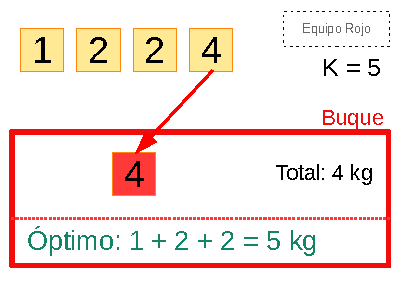
\includegraphics[scale=1]{img/DibCont2.pdf}
    \caption{Ilustración de la maximización del número de toneladas en buque.}
    \label{fig:dib2}
\end{figure}